\graphicspath{{figures/appendix/"Motor&GearTests"/}}
\chapter{Test Journal: Gear Train System}\label{appendix:DCMotorInductance}
\begin{table}[htbp]
\begin{tabular}{l l}
\textbf{Test participants:} & Maxime \& Geoffroy  \\
\textbf{Date:}  & 28/2/2017
\end{tabular}
\end{table}

\section*{Purpose}
The objective of this test is to determine all the of the gear train system composed of the DC motor and the gear train.
\section{Electronics characteristics}

\subsection{Internal Resistance of the DC Motor $R_m$}
The first parameter to be tested is the internal resistance of the motor $R_m$. This resistance is needed in the motor's transfer function and will be used to determine the other parameters of the motor. 
\subsubsection*{Setup}
\autoref{fig:RmMeasurementSetup} shows a diagram and photo of the measurement set up
\begin{figure}[htbp]
	\centering
	\begin{subfigure}{0.50\textwidth}
		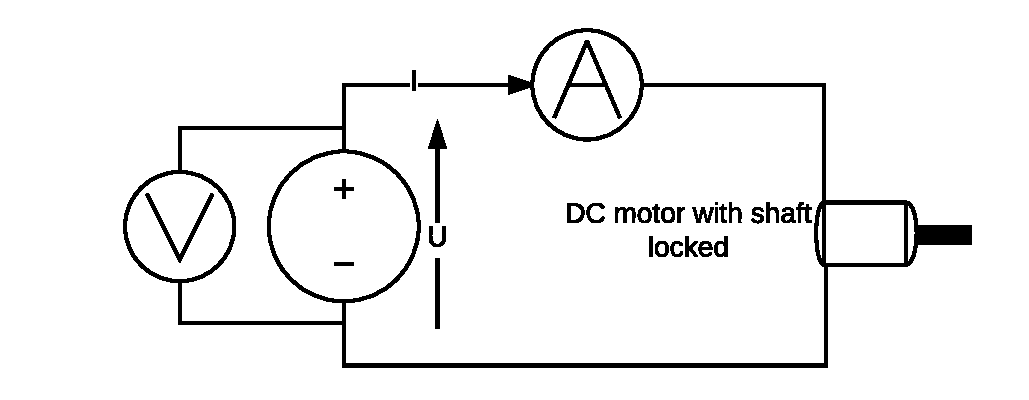
\includegraphics[width=1\textwidth]{figures/appendix/Motor&GearTests/RmTestSetUpDiagram}
		\caption{Diagram of the setup.} \label{fig:LaMeasurementDiagram}
	\end{subfigure}
	\begin{subfigure}{0.40\textwidth}
		\includegraphics[width=1\textwidth]{figures/figureIsComing}
		\caption{Picture of the setup.} \label{fig:LaMeasurementPictures}
	\end{subfigure}
	\caption{The measurement setup.} \label{fig:RmMeasurementSetup}   
\end{figure} 

\subsubsection*{Method}
This test consists of having the motor shaft locked while the voltage is increased by 0.5 V between measurements.

\subsubsection*{Raw data}
\autoref{tab_appendix:RmData} is the plotted evolution of the voltage of the circuit according to the current.

\begin{figure}[htbp]
	\centering
	\caption{Raw data used to determine $R_m$}\label{tab_appendix:RmData}
	\begin{tabularx}{0.35\textwidth}{XX}
		Voltage (V) & Current (A)\\ \toprule \rowcolor{lightGrey}
		0.50 & 0.33 \\
		1.00 & 0.71 \\ \rowcolor{lightGrey}
		1.50 & 1.13 \\
		2.00 & 1.67 \\ \rowcolor{lightGrey}
		2.49 & 2.34 \\
		2.98 & 2.94 \\ \rowcolor{lightGrey}
		3.50 & 3.75 \\
		3.99 & 4.68 \\ \rowcolor{lightGrey}
		4.50 & 5.54 \\
		4.98 & 6.11 \\ \rowcolor{lightGrey}
		5.54 & 6.46 \\
		6.02 & 7.40 \\ \rowcolor{lightGrey}
		6.51 & 8.26 \\
		7.01 & 9.14 
	\end{tabularx}
\end{figure}

\subsubsection{Data Processing}
In order to find the motor's resistance $R_m$, the electrical equations of the motor will be used:
\begin{equation}
	U_m = R_m \cdot i + L_m \frac{di}{dt} + K_e\omega_m
\end{equation}

With the motor shaft locked, $\omega_m = 0$. Moreover, the measurements are made a couple seconds after the change in voltage is made. The current is then constant, canceling its derivative. 

The resulting equation is Ohm's law:
\begin{equation}
U_m = R_m \cdot i
\end{equation}

The measurement of voltage according to the current is presented in \autoref{fig:Rmplot}.
\begin{figure}[htbp]
	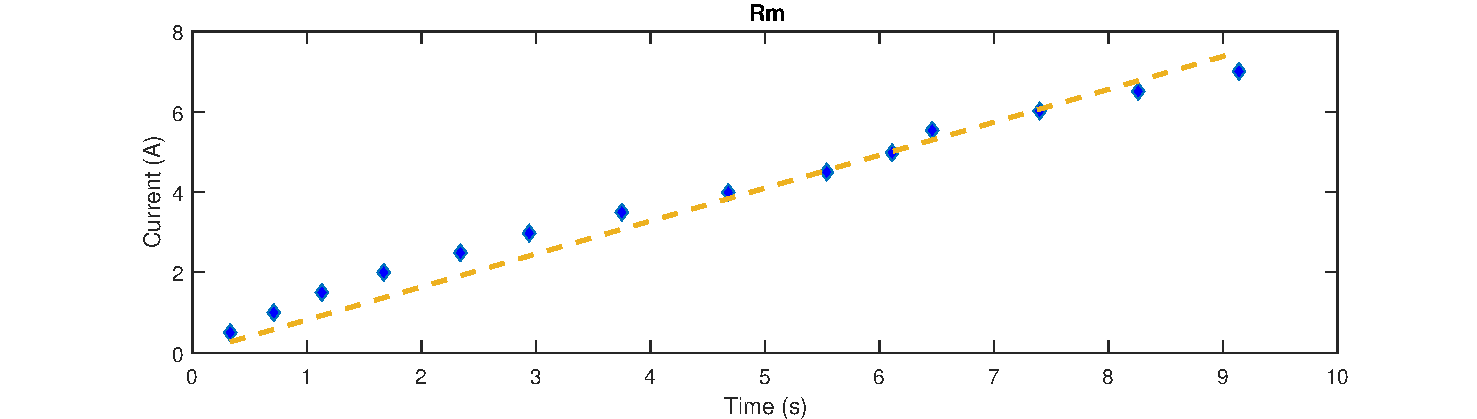
\includegraphics[width=1\textwidth]{figures/modeling/Motor/Rmplot-converted-to-pdf}
	\caption{Diagram of the setup.} \label{fig:Rmplot}
\end{figure}

$R_m$ is the slope of the linear approximation (in dashed yellow) of the voltage over the current: 
\begin{subequations} \label{eq:LaEq}
	\begin{flalign}
		&U_m = R_m \cdot i \\
		&R_m \approx \SI{0.82}{\ohm}
	\end{flalign}
\end{subequations}


\subsection{Internal Inductance of the DC Motor $L_m$}
\begin{table}[htbp]
	\centering
	\caption{List of measurement equipment and components}\label{tab_appendix:LaSetUp}

	\begin{tabularx}{\textwidth}{lXXXX}
		Name 				& Brand	& Model & AAU-number									\\ \toprule \rowcolor{lightGrey}
		Oscilloscope	& Agilent & 54621D & 33941 	\\
		Powersupply	& Agilent & E3631A & 78577\\ \rowcolor{lightGrey}
		DC motor & Alsthom BBC & F9M2& 08339 
	\end{tabularx}
\end{table}
\subsubsection*{Setup}
\autoref{fig:LaMeasurementSetup} shows a diagram and photo of the measurement set up
\begin{figure}[htbp]
	\centering
	\begin{subfigure}{0.50\textwidth}
		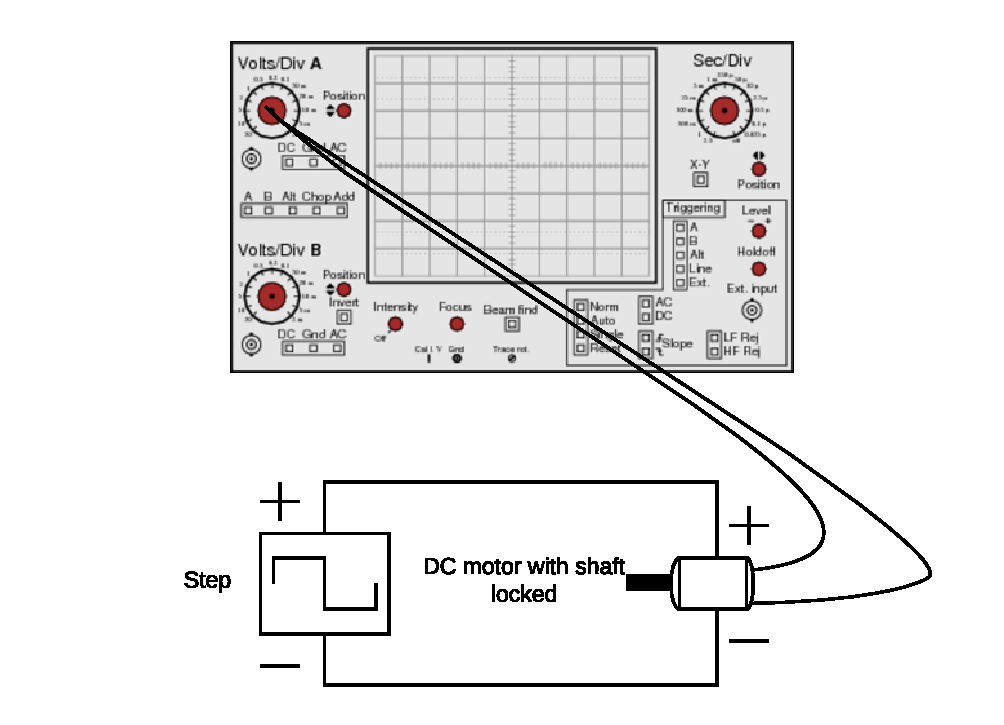
\includegraphics[width=0.7\textwidth]{figures/appendix/Motor&GearTests/LmDiagram}
		\caption{Diagram of the setup.} \label{fig:LaMeasurementDiagram}
	\end{subfigure}
	\begin{subfigure}{0.40\textwidth}
		\includegraphics[width=1\textwidth]{MotorImpedanceTest.jpg}
		\caption{Picture of the setup.} \label{fig:LaMeasurementPictures}
	\end{subfigure}
	\caption{The measurement setup.} \label{fig:LaMeasurementSetup}   
\end{figure}

\subsubsection*{Method}
This test consists of having the motor shaft locked while a step is applied. The voltage of a shunt resistor is then measured by an oscilloscope from which the current is deduced.
\subsubsection*{Raw data}
\autoref{fig:LaTestCurrentPlot} is the plotted evolution of the current of the circuit in respect to time.

%\begin{figure}[htbp]
%	\centering
%	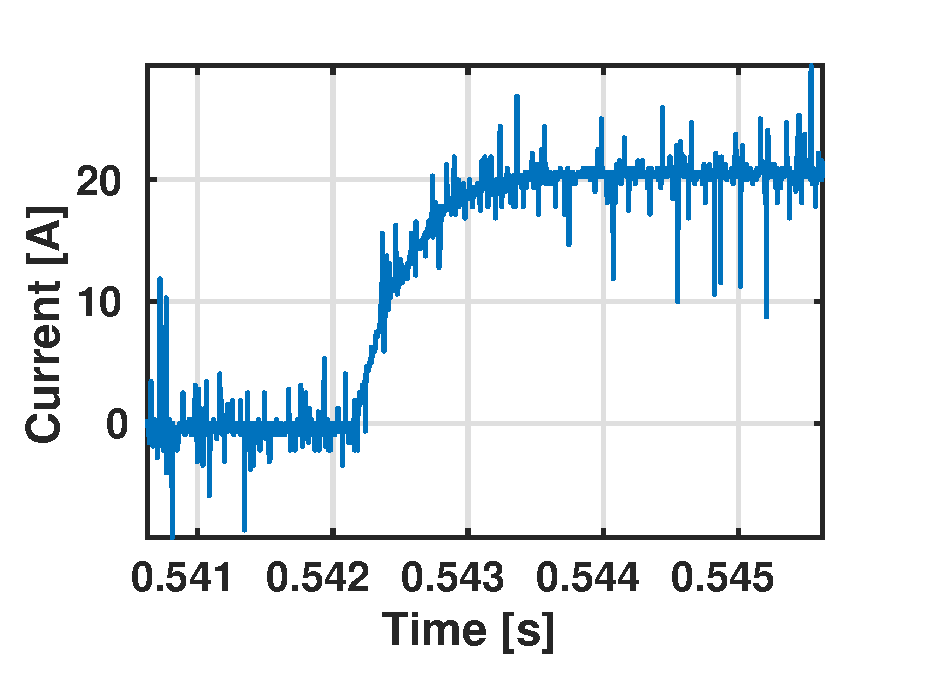
\includegraphics[width=0.7\textwidth]{LaTestCurrentPlot}
%	\caption{Plot of the current in respect to time}\label{fig:LaTestCurrentPlot}
%\end{figure}

\subsubsection*{Data processing}
When the shaft is locked and a step is applied the DC motor's electric equation can be resumed as in \autoref{eq:LaEquation}.
\begin{equation}
	F(s)=\frac{I_a(s)}{U_a(s)}=\frac{\frac{1}{R_a}}{\frac{L_a}{R_a} s+1} \addunit{1}
	\label{eq:LaEquation}
\end{equation}
\startexplain
\explain{$I_a(s)$ is the current in Laplace domain}{1}
\explain{$U_a(s)$ is the body's acceleration}{1}
\explain{$R_a$ is the internal resistance of the motor}{\si{\ohm}}
\explain{$L_a$ is the internal inductance of the motor}{\si{\henry}}
\stopexplain

When a unit step response is applied to the system \autoref{eq:LaEquation} becomes \autoref{eq:LaEquationStep}.

\begin{equation}
F(s)=\frac{\frac{1}{R_a}}{\frac{L_a}{R_a} s+1}\frac{1}{s}=\frac{-\frac{1}{R_a}}{s+\frac{R_a}{L_a}}+\frac{1}{R_a s} \addunit{1}
\label{eq:LaEquationStep}
\end{equation}

\autoref{eq:LaEquationStep} is then put in the continuous time domain to get \autoref{eq:LaEquationStepTime}.

\begin{equation}
f(t)= \frac{1}{R_a} \left(1-e^{-\frac{R_a}{L_a} t}\right) \addunit{1}
\label{eq:LaEquationStepTime}
\end{equation}

\autoref{eq:LaEquationStepTime} means that at $t=\frac{L_a}{R_a}$ the function would give $1-e^{-1}=\SI{63.212055882}{\percent}$ of its settling value. So at \SI{63.212055882}{\percent} of the settling value $t=\frac{L_a}{R_a}$ and since $R_a=\SI{0.43}{\ohm}$ \cite{datasheet:saradc} is known finding $L_a$ becomes trivial.

\subsubsection*{Conclusion}

Since the value of the current at the settling value is \SI{20.471}{\ampere}. Then \autoref{eq:LaEq} gives the value of $L_a$.

\begin{subequations} \label{eq:LaEq}
	\begin{flalign}
		&\frac{1}{R_a} \left(1-e^{-\frac{R_a}{L_a} \tau}\right)=20.471 \cdot 0.63212055882 \addunit{\second} \\
		&t = \SI{0.00190}{\second} \\
		&L_a=tR_a \\
		&L_a=\SI{817}{\micro\henry}
	\end{flalign}
\end{subequations}





\hrule

\hrule

\hrule

\hrule

\hrule

\hrule

SENSTOOL RmLm\\

\begin{table}[htbp]
	\centering
	\caption{List of measurement equipment and components}\label{tab_appendix:LaSetUp}
	
	\begin{tabularx}{\textwidth}{lXXXX}
		Name 				& Brand	& Model & AAU-number									\\ \toprule \rowcolor{lightGrey}
		
		DC motor & Alsthom BBC & F9M2 & 08339 
	\end{tabularx}
\end{table}


\subsubsection*{Setup}
\autoref{fig:KeMeasurementSetup} shows a diagram and photo of the measurement set up

\subsubsection*{Method}
The test will consist of applying a step of \SI{7}{\volt} on the DC motor (which is at \SI{0}{\volt} before that) with its shaft locked. Then via a curve fitting tool named SENSETOOL $R_m$ and $L_m$ are deduced.

\subsubsection*{Raw Data}
The blue line represents the power supply output without load.\\
The gold line is the response of the motor to this step.
\begin{figure}[htbp]
	\centering
	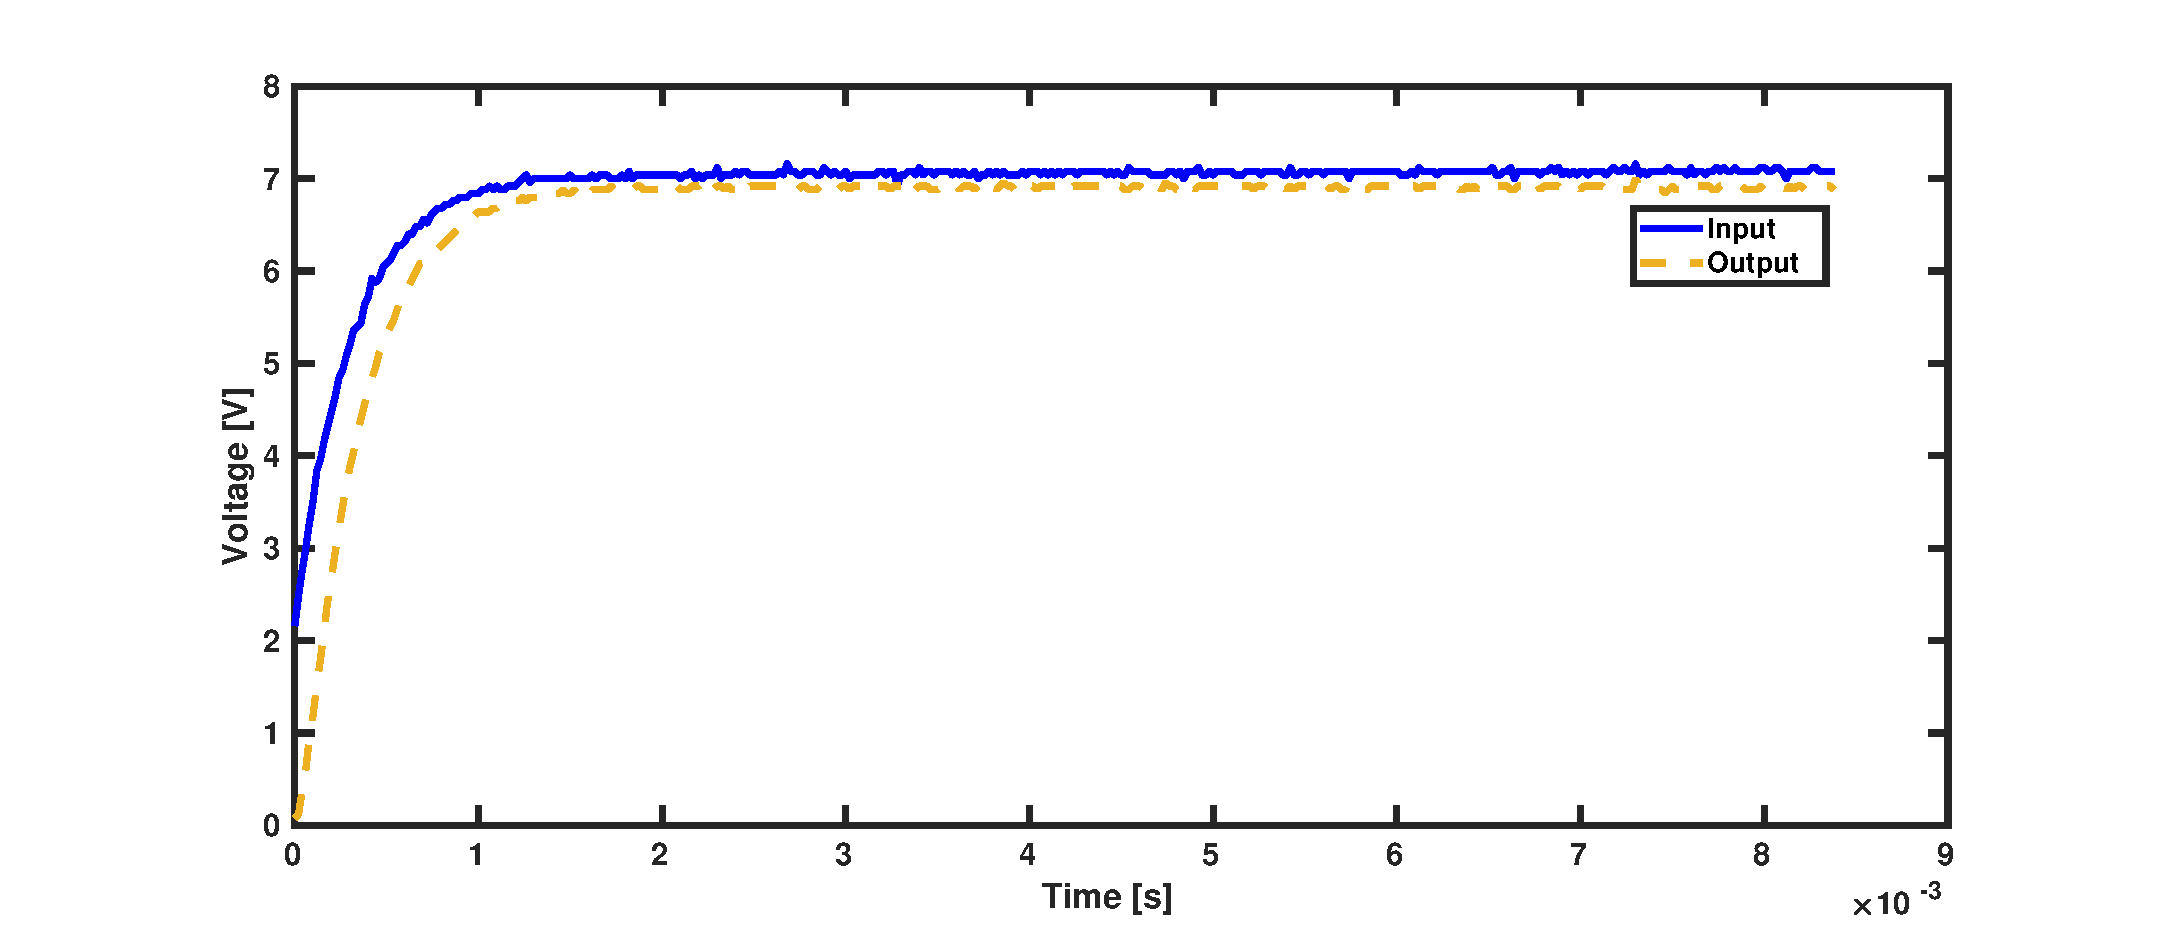
\includegraphics[width=\textwidth]{figures/appendix/Motor&GearTests/RmLmDataPlot}
	\caption{Plot of the voltage in respect to time of the input and the output of the DC motor}\label{fig:RmLmTestDataPlot}
\end{figure}

\subsubsection*{Data processing}

Since the shaft is locked, a step is applied and only the electrical characteristics of the motor are looked at. The data measured follows \autoref{eq:RmLmChar}.

\begin{equation} \label{eq:RmLmChar}
	u(t)=R_m i(t)+L_m \frac{d i(t)}{d t} \addunit{\volt}
\end{equation}

Which gives the transfer function \autoref{eq:RmLmTf}. Which is used to find $R_m$ and $L_m$ by curve fitting.

\begin{equation} \label{eq:RmLmTf}
\frac{I(s)}{U(s)}=\frac{1}{R_m +L_m s} \addunit{1}
\end{equation}

\subsubsection*{Conclusion}

After the curve fitting the following values are found $R_m=\SI{1.02}{\ohm}$ and $L_m=\SI{142}{\micro\henry}$. \autoref{fig:RmLmTestFitPlot} is a comparison between the model with these parameters and the measures done.

\begin{figure}[htbp]
	\centering
	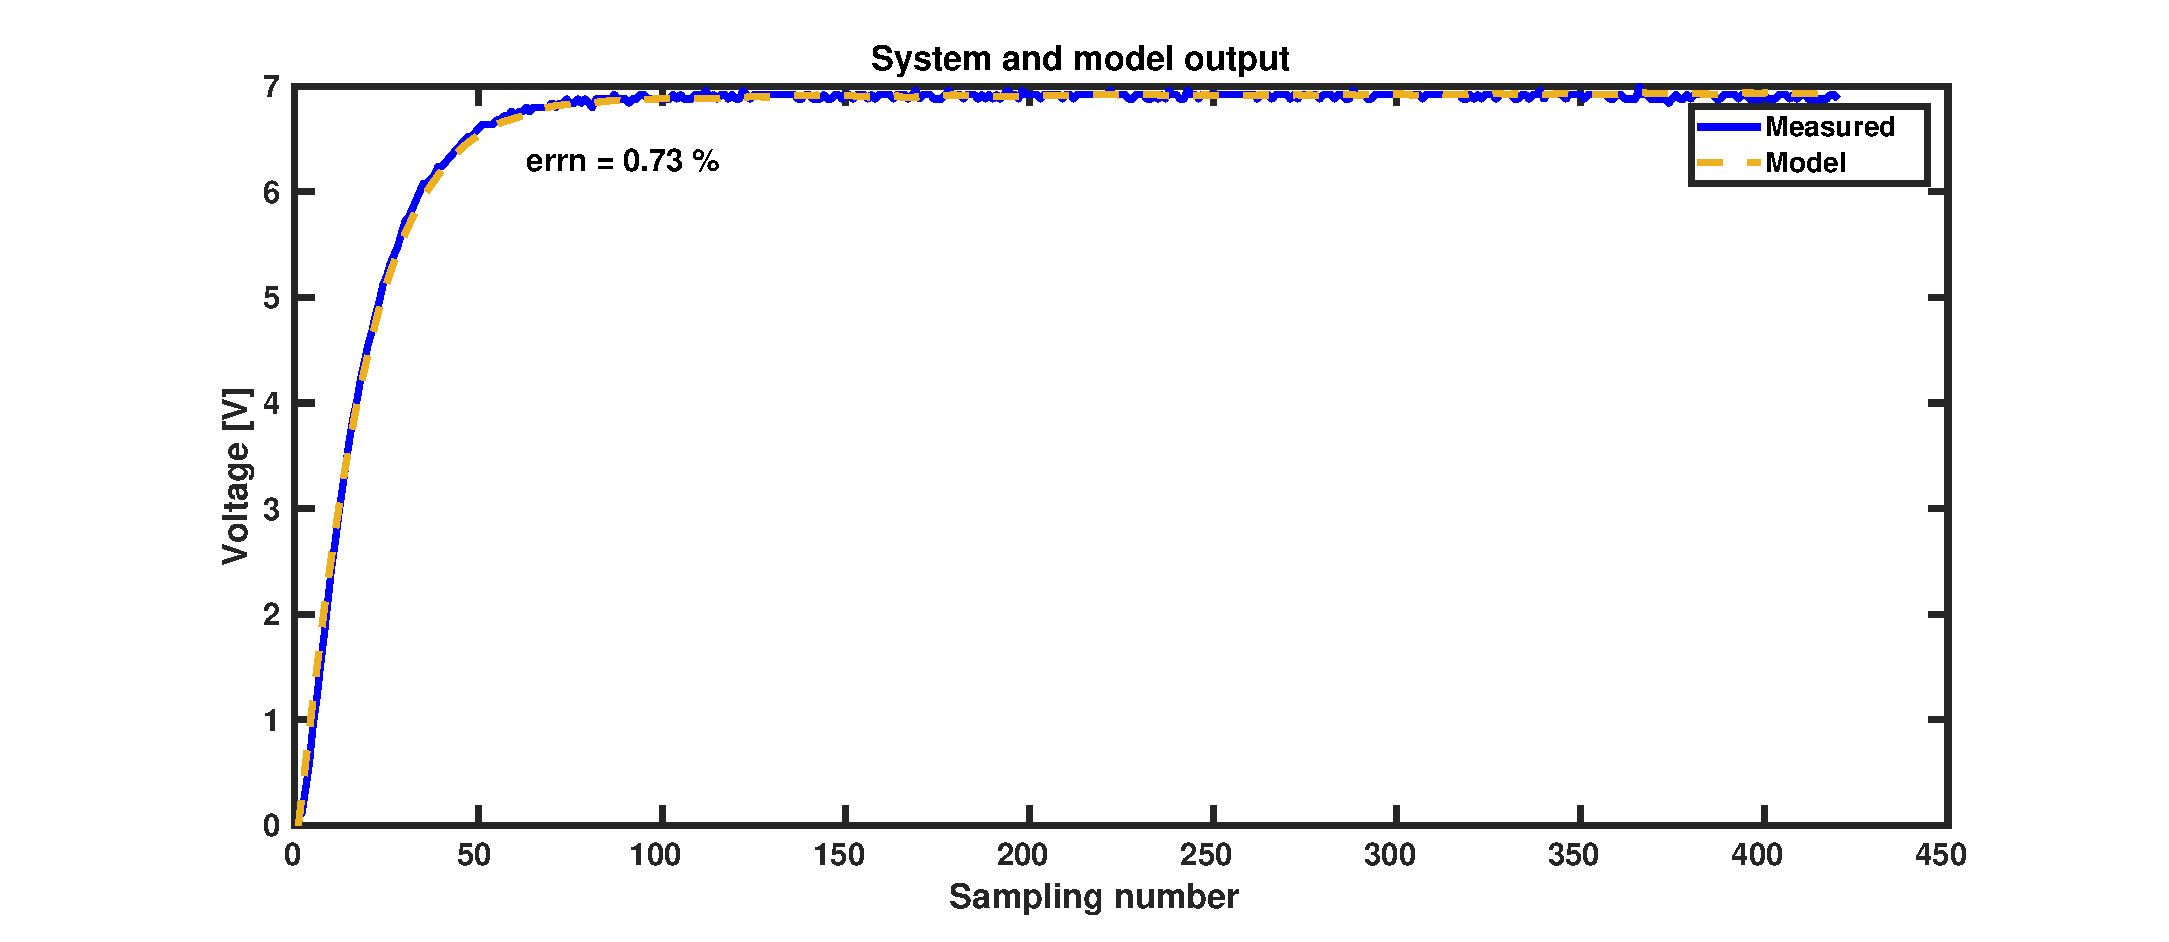
\includegraphics[width=\textwidth]{figures/appendix/Motor&GearTests/RmLmFitPlot}
	\caption{Plot of the comparison between the model and the measures}\label{fig:RmLmTestFitPlot}
\end{figure}
\hrule

\hrule

\hrule

\hrule

\hrule

\hrule


\subsection{The DC Motor velocity constant $K_e$}
\begin{table}[htbp]
	\centering
	\caption{List of measurement equipment and components}\label{tab_appendix:KeSetUp}
	
	\begin{tabularx}{\textwidth}{lXXXX}
		Name 				& Brand	& Model & AAU-number									\\ \toprule \rowcolor{lightGrey}
		Oscilloscope	& Agilent & 54621D & 33941 	\\
		Powersupply	& Agilent & E3631A & 78577\\ \rowcolor{lightGrey}
		DC motor & Alsthom BBC & F9M2& 08339
	\end{tabularx}
\end{table}

\subsubsection*{Setup}
\autoref{fig:KeMeasurementSetup} shows a diagram and photo of the measurement set up
\begin{figure}[htbp]
	\centering
	\begin{subfigure}{0.50\textwidth}
		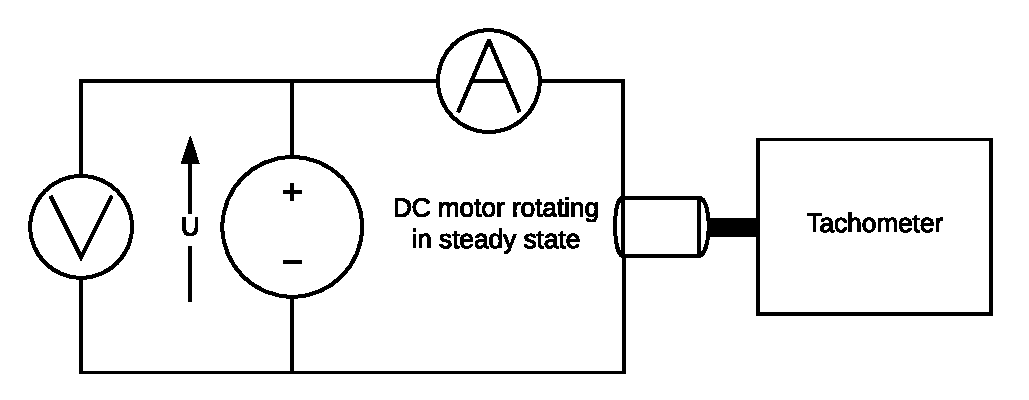
\includegraphics[width=\textwidth]{figures/appendix/Motor&GearTests/KeTestSetUp}
		\caption{Diagram of the set up.} \label{fig:KeMeasurementDiagram}
	\end{subfigure}
	\begin{subfigure}{0.40\textwidth}
		\includegraphics[width=1\textwidth]{figures/appendix/Motor&GearTests/KeTestPic}
		\caption{Picture of the set up.} \label{fig:KeMeasurementPictures}
	\end{subfigure}
	\caption{The measurement set up for $K_e$.} \label{fig:KeMeasurementSetup}   
\end{figure}

\subsubsection*{Method}
This test consists of having the motor shaft rotating in steady state while the voltage $U$ of the generator, the angular velocity $\omega$ of the shaft and the current $I$ are measured.

\subsubsection*{Raw data}
\autoref{tab_appendix:KeData} has all the measurements done.
\begin{figure}[htbp]
	\centering
	\caption{Raw data used to determine $K_e$}\label{tab_appendix:KeData}
	\begin{tabularx}{0.55\textwidth}{lXX}
		Voltage (V) & Current (A) & $\omega$ (rad/s)\\ \toprule \rowcolor{lightGrey}
		3.0  & 0.72 & 52.36  \\
		3.5  & 0.75 & 67.54  \\ \rowcolor{lightGrey}
		4.0  & 0.77 & 83.15  \\
		4.5  & 0.79 & 98.75  \\ \rowcolor{lightGrey}
		5.0  & 0.83 & 113.10 \\
		5.5  & 0.85 & 126.71 \\ \rowcolor{lightGrey}
		6.0  & 0.88 & 140.95 \\
		6.5  & 0.90 & 156.03 \\ \rowcolor{lightGrey}
		7.0  & 0.93 & 170.38 \\
		7.5  & 0.94 & 185.35 \\ \rowcolor{lightGrey}
		8.0  & 0.95 & 198.97 \\
		8.5  & 0.96 & 214.68 \\ \rowcolor{lightGrey}
		9.0  & 0.99 & 229.34 \\
		9.5  & 1.00 & 244.31 \\ \rowcolor{lightGrey}
		10.0 & 1.02 & 258.66 \\
		10.5 & 1.03 & 274.05 \\ \rowcolor{lightGrey}
		11.0 & 1.06 & 289.03 \\
		11.5 & 1.06 & 304.73 \\ \rowcolor{lightGrey}
		12.0 & 1.05 & 321.49
	\end{tabularx}
\end{figure}



\subsubsection*{Data processing}

When the shaft is rotating in steady state as shown in \autoref{fig:KeMeasurementDiagram}, \autoref{eq:KeSetUpElec} can be derived.
\begin{equation}
U=K_e\omega+R_m I \addunit{\volt}
\label{eq:KeSetUpElec}
\end{equation}

\startexplain
\explain{$I$ is the current in the circuit}{\si{\ampere}}
\explain{$U$ is the generator's voltage}{\si{\volt}}
\explain{$K_e$ is the velocity constant of the motor}{\si{\volt\per\radian\second}}
\explain{$R_m$ is the internal resistance of the motor}{\si{\ohm}}
\stopexplain

From \autoref{eq:KeSetUpElec} \autoref{eq:KeForm} is obtained by isolating $K_e$.

\begin{equation}
K_e=\frac{U-R_m I}{\omega} \addunit{\volt\per\radian\second}
\label{eq:KeForm}
\end{equation}

\subsubsection*{Conclusion}

\autoref{fig:KeTest} plot the $K_e$ found for each measurement. The $K_e$ used in the model is average of these points. This gives $K_e=\SI{0.0343}{\volt\per\radian\second}$

\begin{figure}[htbp]
	\centering
	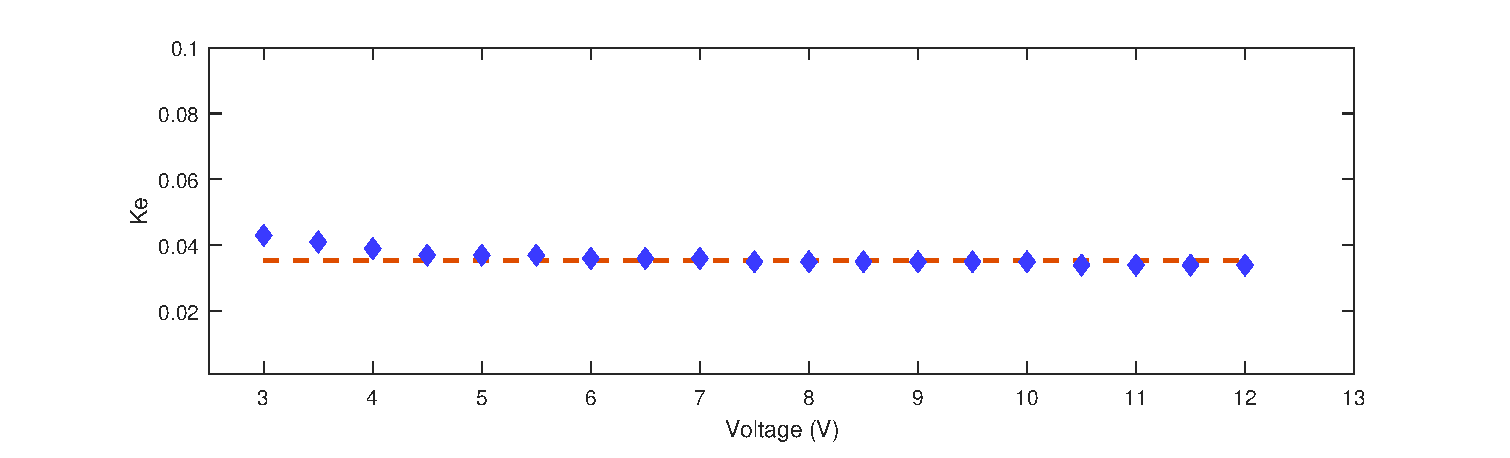
\includegraphics[width=1.1\textwidth]{figures/appendix/Motor&GearTests/PlotKe}
	\caption{Plot of $K_e$ found for each measures}\label{fig:KeTest}
\end{figure}


\subsection{The DC Motor torque constant $K_t$}
\begin{table}[htbp]
	\centering
	\caption{List of measurement equipment and components}\label{tab_appendix:KtSetUp}
	
	\begin{tabularx}{\textwidth}{lXXXX}
		Name 				& Brand	& Model & AAU-number									\\ \toprule \rowcolor{lightGrey}
		Oscilloscope	& Agilent & 54621D & 33941 	\\
		Powersupply	& Agilent & E3631A & 78577\\ \rowcolor{lightGrey}
		DC motor & Alsthom BBC & F9M2& 08339
	\end{tabularx}
\end{table}

\subsubsection*{Setup}
\autoref{fig:KtMeasurementSetup} shows a diagram and photo of the measurement set up
\begin{figure}[htbp]
	\centering
	\begin{subfigure}{0.50\textwidth}
			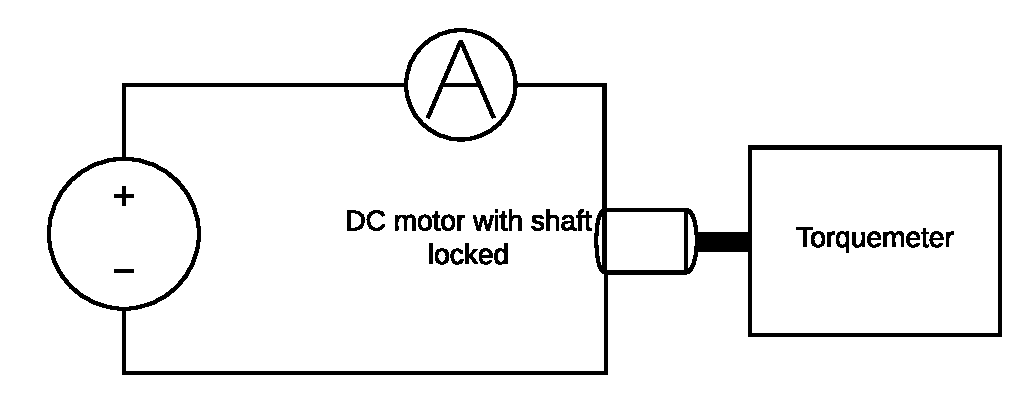
\includegraphics[width=\textwidth]{KtTestSetUp}
		\caption{Diagram of the setup.} \label{fig:KtMeasurementDiagram}
	\end{subfigure}
	\begin{subfigure}{0.40\textwidth}
		%\includegraphics[width=1\textwidth]{MotorImpedanceTest.jpg}
		\missingfigure{Picture of the setup}
		\caption{Picture of the setup.} \label{fig:KtMeasurementPictures}
	\end{subfigure}
	\caption{The measurement setup.} \label{fig:KtMeasurementSetup}   
\end{figure}

\subsubsection*{Method}
This test consists of having the motor shaft locked while the torque $\tau_m$ and the current $I$ are measured.

\subsubsection*{Raw data}
\autoref{tab:KtTest} has all the measurements done.


\subsubsection*{Data processing}

When the motor is in steady state and the shaft locked as shown in \autoref{fig:KtMeasurementDiagram}, \autoref{eq:KtTest} is found from \autoref{eq:MotorTorque}.

\begin{equation}\label{eq:KtTest}
K_t=\frac{\tau_m}{I} \addunit{\newton\meter\per\ampere}
\end{equation}
\startexplain
\explain{$I$ is the current in the circuit}{\si{\ampere}}
\explain{$\tau_m$ is the torque of the motor}{\si{\newton\meter}}
\explain{$K_t$ is the motor's torque constant}{\si{\newton\meter\per\ampere}}
\stopexplain

\subsubsection*{Conclusion}

\autoref{fig:KtTest} plot the $K_t$ found for each measurement. The $K_t$ used in the model is average of these points. This gives $K_t=\SI{0.025}{\newton\meter\per\ampere}$

\begin{figure}[htbp]
	\centering
	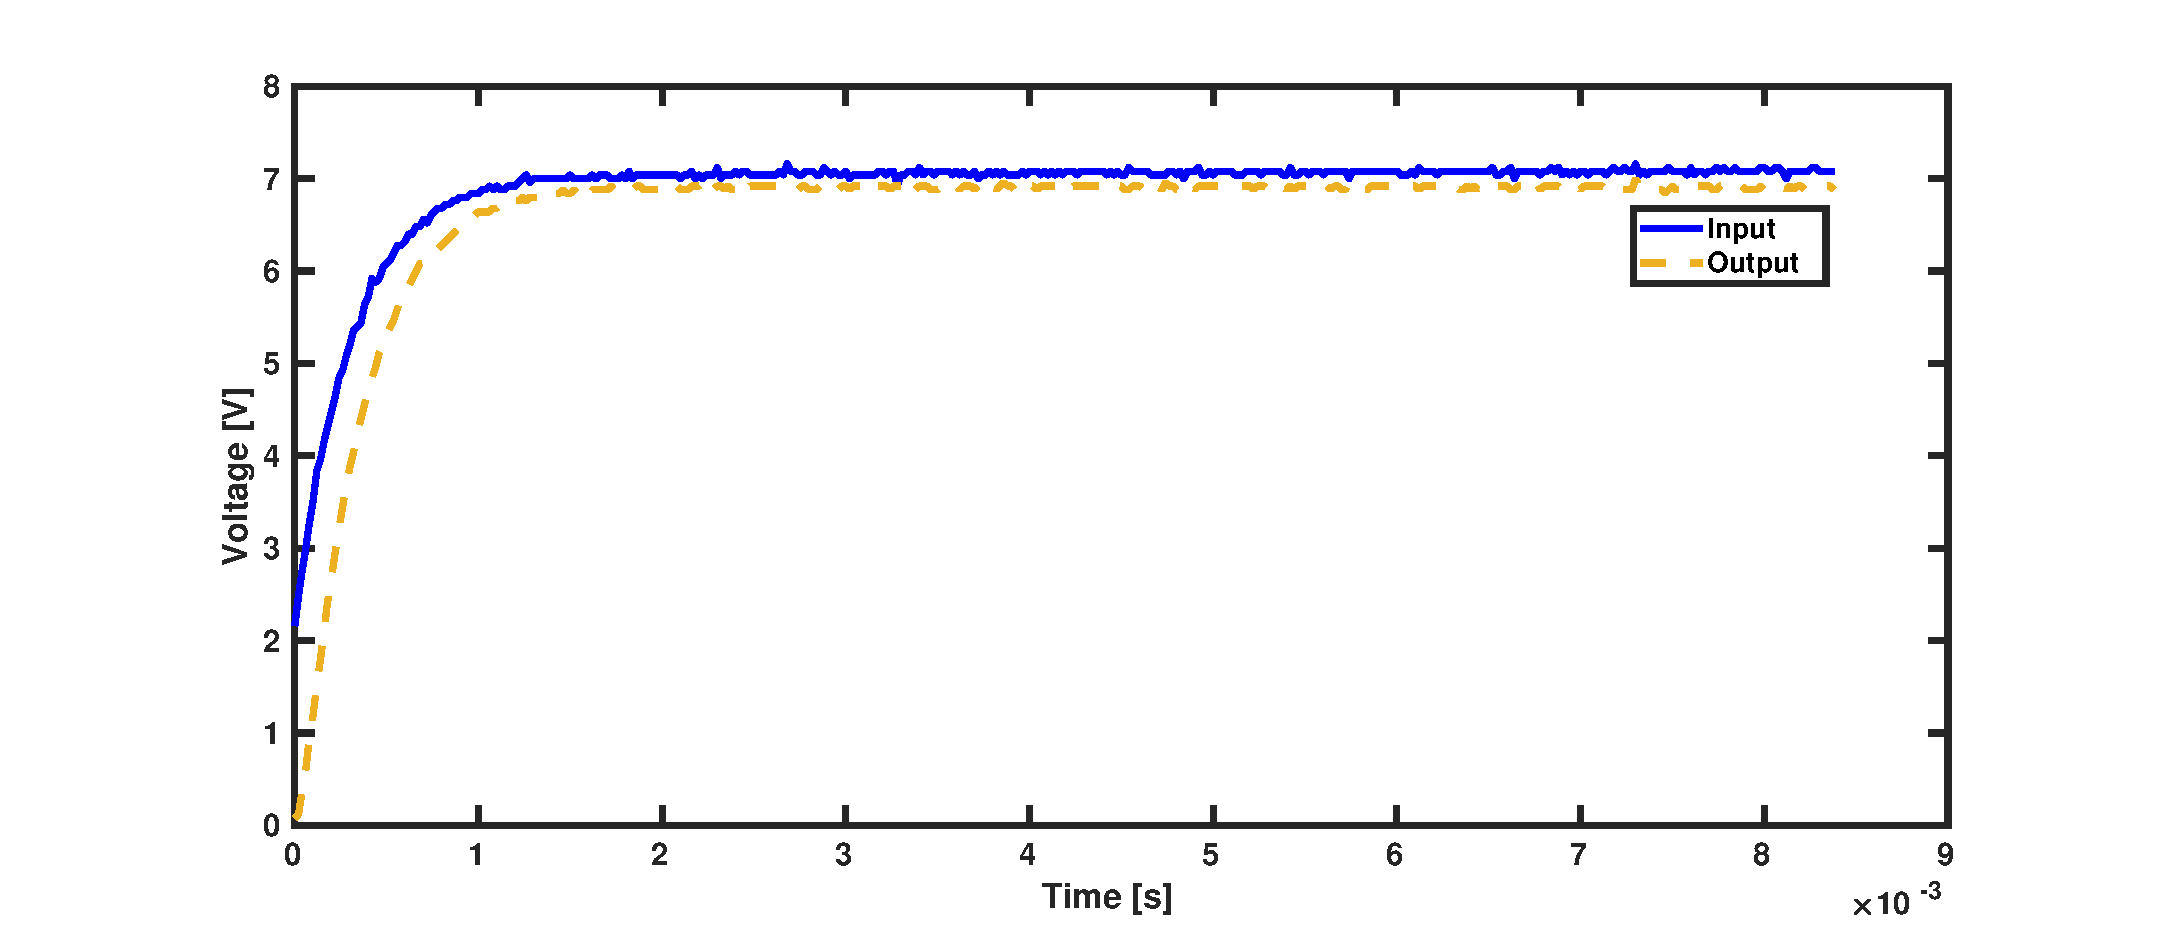
\includegraphics[width=\textwidth]{figures/appendix/Motor&GearTests/RmLmDataPlot}
	\caption{Plot of $K_e$ found for each measures}\label{fig:KtTest}
\end{figure}

\section{Mechanical Characteristics}

\subsection{Frictions $B_m$}
\begin{table}[htbp]
	\centering
	\caption{List of measurement equipment and components}\label{tab_appendix:BmSetUp}
	
	\begin{tabularx}{\textwidth}{lXXXX}
		Name 				& Brand	& Model & AAU-number									\\ \toprule \rowcolor{lightGrey}
		Oscilloscope	& Agilent & 54621D & 33941 	\\
		Powersupply	& Agilent & E3631A & 78577\\ \rowcolor{lightGrey}
		DC motor & Alsthom BBC & F9M2& 08339
	\end{tabularx}
\end{table}

\subsubsection*{Setup}
\autoref{fig:BmMeasurementSetup} shows a diagram and photo of the measurement set up
\begin{figure}[htbp]
	\centering
	\begin{subfigure}{0.50\textwidth}
		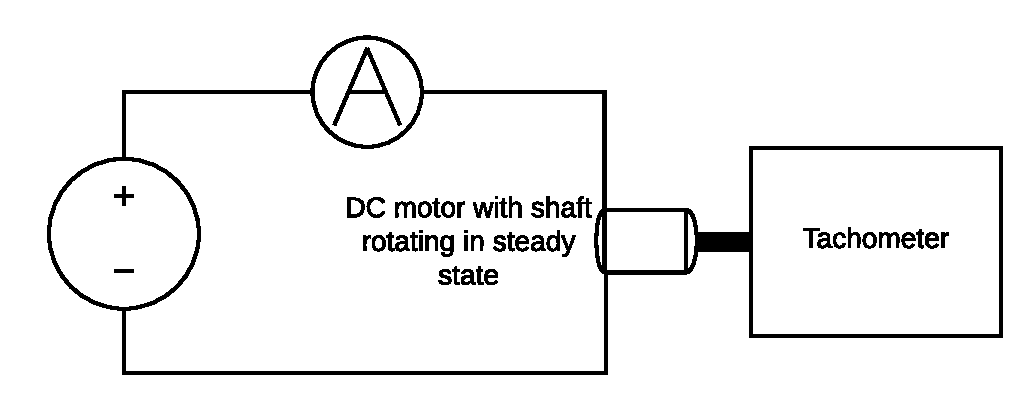
\includegraphics[width=\textwidth]{BmTestSetUp}
		\caption{Diagram of the set up.} \label{fig:BmMeasurementDiagram}
	\end{subfigure}
	\begin{subfigure}{0.40\textwidth}
		%\includegraphics[width=1\textwidth]{MotorImpedanceTest.jpg}
		\missingfigure{Picture of the setup}
		\caption{Picture of the setup.} \label{fig:BmMeasurementPictures}
	\end{subfigure}
	\caption{The measurement set up.} \label{fig:BmMeasurementSetup}   
\end{figure}

\subsubsection*{Method}
This test consists of having the motor shaft running in steady state while the torque $\tau_m$, the shaft angular velocity $\omega$ and the current $I$ are measured.

\subsubsection*{Raw data}
\autoref{tab:KtTest} has all the measurements done.


\subsubsection*{Data processing}

The motor and the shaft are in steady state so $\tau_m=\tau_{fm}$ which combined with \autoref{eq:FrictionTorque} gives \autoref{eq:BmTest}.

\begin{equation}\label{eq:BmTest}
B_m=\frac{K_t I}{\omega} \addunit{\newton\per\radian\second}
\end{equation}
\startexplain
\explain{$I$ is the current in the circuit}{\si{\ampere}}
\explain{$K_t$ is the motor's torque constant}{\si{\newton\meter}}
\explain{$\omega$ is the shaft's angular velocity}{\si{\radian\per\second}}
\explain{$B_m$ is the viscous friction constant}{\si{\newton\per\radian\second}}
\stopexplain

\subsubsection*{Conclusion}

\autoref{fig:BmTest} plot the $B_m$ found for each measurement. The $B_m$ used in the model is average of these points. This gives $B_m=\SI{120}{\micro\newton\per\radian\second}$

\begin{figure}[htbp]
	\centering
	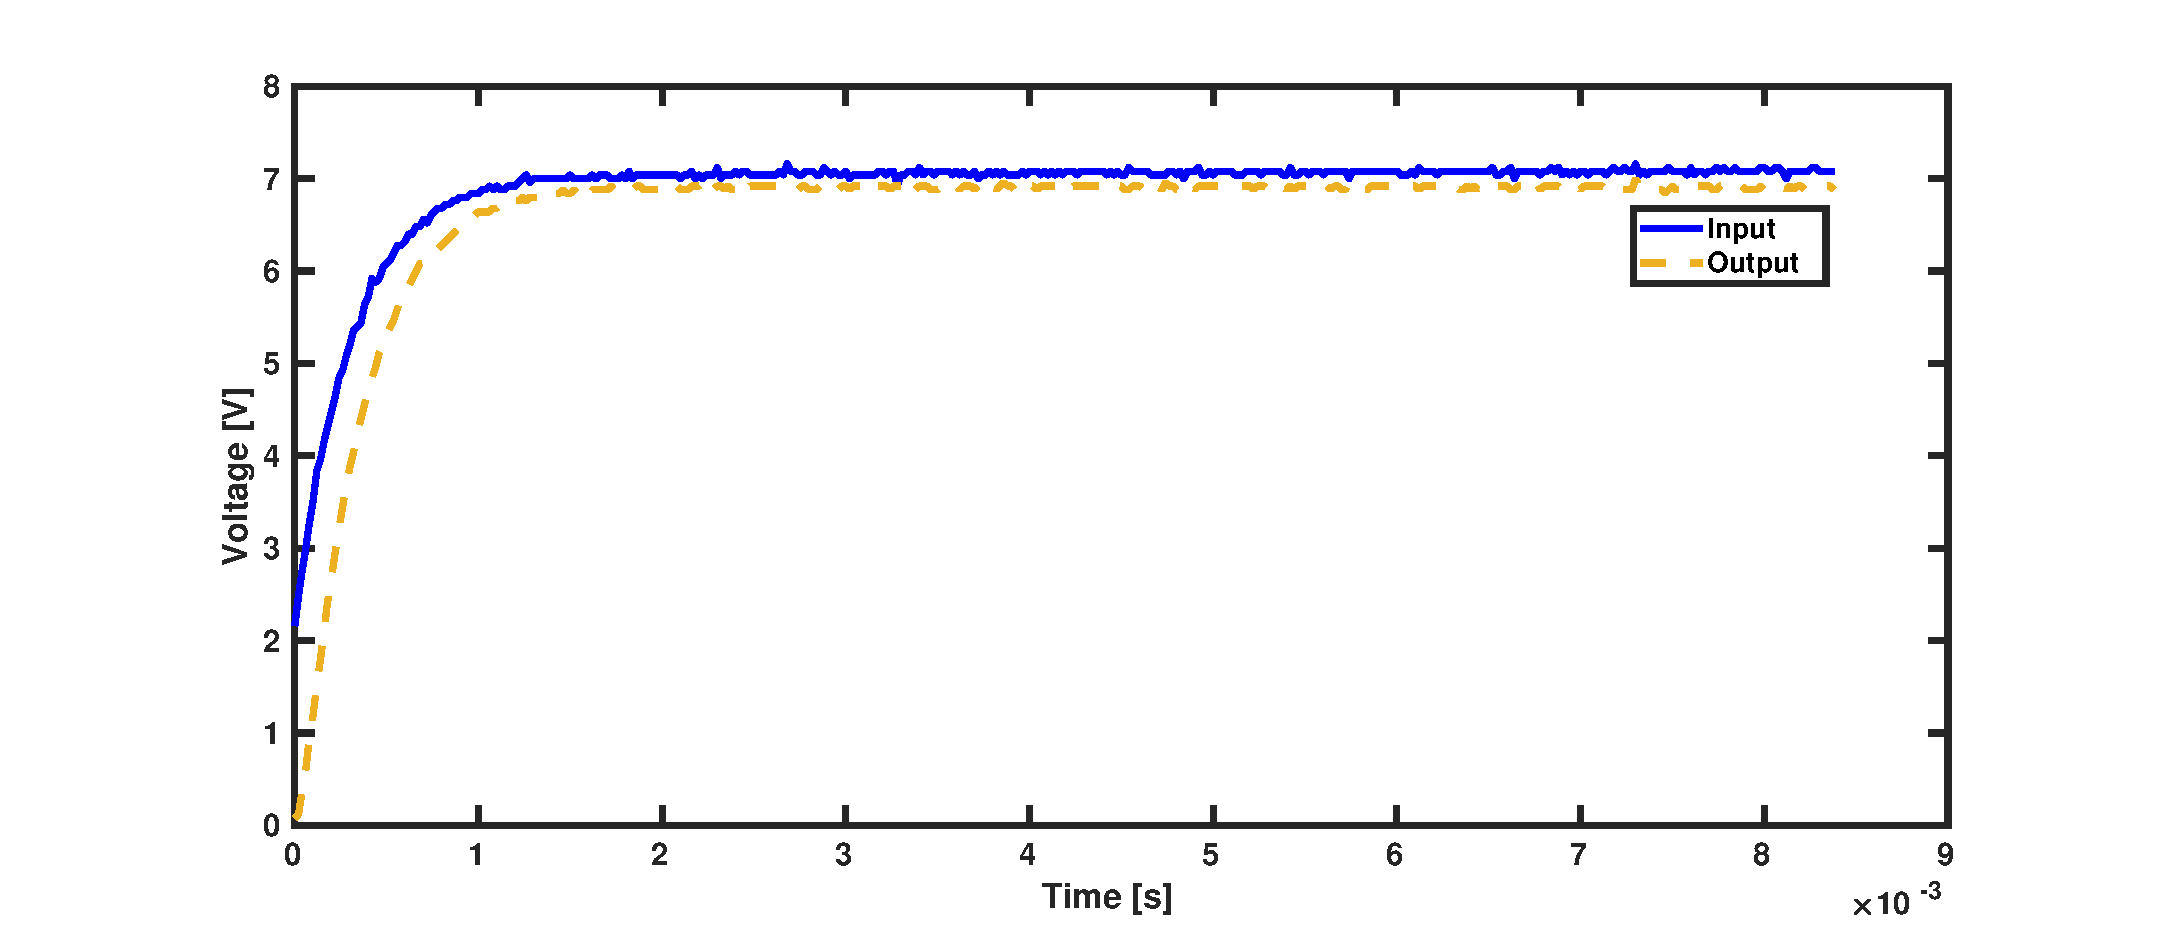
\includegraphics[width=\textwidth]{figures/appendix/Motor&GearTests/RmLmDataPlot}
	\caption{Plot of $B_m$ found for each measures}\label{fig:BmTest}
\end{figure}
\break

\subsection{Moment of Inertia of the Gears $J_gear$}

The moment of inertia of the gear train was thoroughly calculated in a previous report and will be used here.

\subsubsection*{Method}
The gear train can by divided in three parts: the large wheels, the small wheels and the axles. The latter is a solid cylinder whereas the wheels are considered as multiple hollowed cylinders. The moment of inertia about a symmetry axis through the center of mass for a hollow cylinder is described in \autoref{eq:MomentInertiaHollowedCylinder}: 
\begin{equation}
	J_{hc} = \frac{1}{2} M (R_1^2 + R_2^2)
	\label{eq:MomentInertiaHollowedCylinder}
\end{equation}
\startexplain
\explain{$J_{hc}$ is the moment of inertia about a symmetry axis through the center of mass for a hollow cylinder}{\si{\kilo\gram\meter\squared}}
\explain{$M$ is the mass of the hollowed cylinder}{\si{\kilo\gram}}
\explain{$R_1$ is the inner radius of the hollowed cylinder}{\si{\meter}}
\explain{$R_2$ is the outer radius of the hollowed cylinder}{\si{\meter}}
\stopexplain

For the axles, the inner radius $R_1$ is equal to zero, giving equation \autoref{eq:MomentInertiaSolidCylinder} for the solid cylinder.
\begin{equation}
	J_{sc} = \frac{1}{2} M R^2
	\label{eq:MomentInertiaSolidCylinder}
\end{equation}
\startexplain
\explain{$J_{sc}$ is the moment of inertia about a symmetry axis through the center of mass for a solid cylinder}{\si{\kilo\gram\meter\squared}}
\explain{$M$ is the mass of the solid cylinder}{\si{\kilo\gram}}
\explain{$R$ is the inner radius of the solid cylinder}{\si{\meter}}
\stopexplain

The mass of each wheels and axles are calculated using their volumes and the density of iron.

\begin{figure}[htbp]
    \centering
    \begin{minipage}[t]{0.45\textwidth}
        \centering
        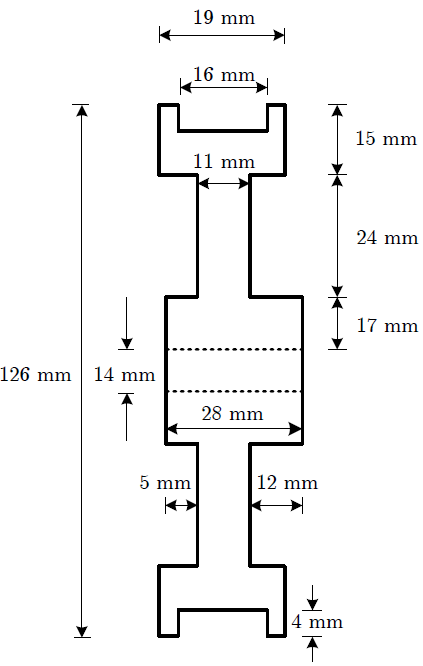
\includegraphics[width=0.9\textwidth]{figures/appendix/Motor&GearTests/BigWheel} 
        \caption{Cross section of a large wheel \citep{web:BalancingStick2008}.}
    \end{minipage}\hfill
    \begin{minipage}[t]{0.45\textwidth}
        \centering
        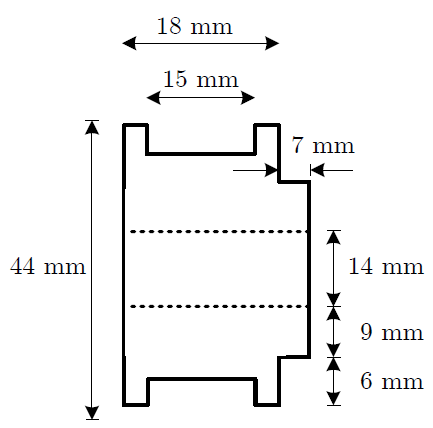
\includegraphics[width=0.9\textwidth]{figures/appendix/Motor&GearTests/SmallWheel} 
        \caption{Cross section of a small wheel \citep{web:BalancingStick2008}.}
    \end{minipage}
\end{figure}

\subsubsection*{Conclusion}
The moment of inertia for each part of the gear system \citep{web:BalancingStick2008}:
\begin{subequations} \label{eq:ResumeMomentInertiaGears}
	\begin{flalign}
		\text{Large Wheel: } J_{Large} &= 1.433 \cdot 10^{-3} \ \si{\kilo\gram\meter\squared} \\
		\text{Small Wheel: } J_{Small} &= 0.037 \cdot 10^{-3}\ \si{\kilo\gram\meter\squared} \\
		\text{Axle 1: }\quad J_{A1} &= 0.083 \cdot 10^{-3}\ \si{\kilo\gram\meter\squared} \\
		\text{Axle 2: }\quad J_{A2} &= 0.078 \cdot 10^{-3}\ \si{\kilo\gram\meter\squared} \\
		\text{Axle 3: }\quad J_{A3} &= 0.092 \cdot 10^{-3}\ \si{\kilo\gram\meter\squared} 
	\end{flalign}
\end{subequations}

The total moment of inertia of the gear system can be calculated from \autoref{eq:TaufReorganized} in \autoref{sec:ModGearSys}.
\begin{equation}
	J_{gear} = N^2J_1 + N^4J_2 + N^6J_3
\end{equation}

With:
\begin{subequations} \label{eq:J1J2J3}
	\begin{flalign}
		J_{1} \:&=\: J_{Large} + J_{Small} + J_{A1} \:=\: 1.553 \cdot 10^{-3}\ \si{\kilo\gram\meter\squared} \\
		J_{2} \:&=\: J_{Large} + J_{Small} + J_{A2} \:=\: 1.548 \cdot 10^{-3}\ \si{\kilo\gram\meter\squared} \\
		J_{3} \:&=\: J_{Large} + J_{Small} + J_{A3} \:=\: 1.562 \cdot 10^{-3}\ \si{\kilo\gram\meter\squared} 
	\end{flalign}
\end{subequations}

Finally, $J_{gear}$ is calculated to be
\begin{equation}
	J_{gear} = 0.153 \cdot 10^{-3}\ \si{\kilo\gram\meter\squared}
\end{equation}



